\documentclass[aspectratio=169, 10pt]{beamer}
\usetheme[progressbar=frametitle]{metropolis}
\usefonttheme{serif}

\usepackage{lmodern}

\usepackage{graphicx}
\usepackage{amssymb}
\usepackage{amsmath}
\usepackage{latexsym}
\usepackage{xcolor}
\usepackage{hyperref}
\usepackage{adjustbox}
\usepackage{mathtools}

\usepackage{multicol}

\usepackage{svg}
\svgpath{{figures/}}

\usepackage{tikz}

% externalize tikz figures to speed up compilation
% \usetikzlibrary{external}
% \tikzexternalize
% \tikzsetexternalprefix{compiled_figures/}
% \tikzexternalize[only named pictures=true]

\usetikzlibrary{arrows, arrows.meta, positioning, shapes.geometric, calc, decorations.pathreplacing, fit}
\usetikzlibrary{backgrounds}
\usetikzlibrary{positioning}
\usetikzlibrary{overlay-beamer-styles}
\usetikzlibrary{angles, quotes}


% 3d tikz
\usepackage{tikz-3dplot}


\definecolor{PGAred}{HTML}{C30A3A}
\definecolor{PGAblue}{HTML}{1482C8}
\definecolor{PGAgreen}{HTML}{1482C8}
\definecolor{PGAyellow}{HTML}{1482C8}


\input{colors}

%%%%%%%%%%%%%%%%%%%%%%%%%%%%%%%%%%%%%%%%%%%%%%%%%%%%%%%%%%%%%%%%%%%%%%%%%%%%%%%%%%%%%%%%%%%%%%%%%
\title{Projective Geometric Algebra\\powers up Bézier Curves}
\institute[LIGM \& LAMA]{LIGM, Université Gustave Eiffel \quad LAMA, Université Savoie Mont-Blanc, CNRS}
\author[Harquin et al.]{\small \textbf{Enzo Harquin}$^1$, Stéphane Breuils$^2$, Venceslas Biri$^1$, Vincent Nozick$^1$}
\date{\alert{WSCG 2026}}
%%%%%%%%%%%%%%%%%%%%%%%%%%%%%%%%%%%%%%%%%%%%%%%%%%%%%%%%%%%%%%%%%%%%%%%%%%%%%%%%%%%%%%%%%%%%%%%%%


%%%%%%%%%%%%%%%%%%%%%%%%%%%%%%%%%%%%%%%%%%%%%%%%%%%%%%%%%%%%%%%%%%%%%%%%%%%%%%%%%%%%%%%%%%%%%%%%%
\begin{document}


% ============================================================================
% BLOCK A — TITLE & MOTIVATION
% ============================================================================

%%%%%%%%%%%%%%%%%%%%%%%%%%%%%%%%%%%%%%%%%%%%%%%%%%%%%%%%%%%%%%%%%%%%%%%%%%%%%%%%%%%%%%%%%%%%%%%%%
\begin{frame}
  \titlepage
\end{frame}
%%%%%%%%%%%%%%%%%%%%%%%%%%%%%%%%%%%%%%%%%%%%%%%%%%%%%%%%%%%%%%%%%%%%%%%%%%%%%%%%%%%%%%%%%%%%%%%%%


% \begin{frame}[t]{Why PGA for Bézier Curves?}
%     \setlength{\columnsep}{20pt}
%     \begin{columns}[T]

%         \column{0.48\textwidth}

%         \textbf{Classical rational Bézier:} points $P_i$ with weights $w_i$ in homogeneous coordinates.

%         \vspace{0.2cm}
%         Limitations:
%         \begin{itemize}\setlength\itemsep{0.1em}
%             \item Interpolates only \alert{points}; lines, planes, conics need ad-hoc constructions
%             \item Projective interactions handled \alert{externally}, not natively
%             \item \alert{Negative weights} avoided: uncontrolled singularities
%             \item \alert{Ideal points} require special cases
%         \end{itemize}

%         \vspace{0.15cm}
%         \alert{\textbf{PGA}} unifies points, ideal points, lines, planes, and rigid transforms under the \emph{same} blending equation.

%         \column{0.52\textwidth}

%         \begin{minipage}[c][0.8\textheight][c]{\linewidth}
%             \centering
%             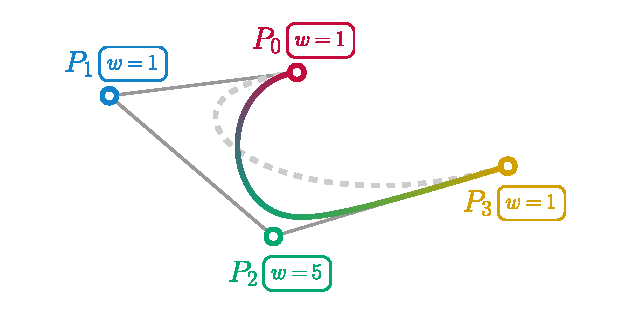
\includegraphics[width=\linewidth]{figures/3_2_cubic_rational_bezier_curve.pdf}\\[0.15cm]
%             {\small Cubic rational Bézier curve}
%         \end{minipage}

%     \end{columns}
% \end{frame}
%%%%%%%%%%%%%%%%%%%%%%%%%%%%%%%%%%%%%%%%%%%%%%%%%%%%%%%%%%%%%%%%%%%%%%%%%%%%%%%%%%%%%%%%%%%%%%%%%


% ============================================================================
% BLOCK B — BACKGROUND
% ============================================================================

%%%%%%%%%%%%%%%%%%%%%%%%%%%%%%%%%%%%%%%%%%%%%%%%%%%%%%%%%%%%%%%%%%%%%%%%%%%%%%%%%%%%%%%%%%%%%%%%%
\begin{frame}[t]{Classical Bézier Curves}
    \setlength{\columnsep}{20pt}
    \begin{columns}[T]

        \column{0.55\textwidth}

        \textbf{Polynomial Bézier} \textcolor{gray}{(degree $d$)}:
        \[
            \textstyle P(t) = \displaystyle\sum_{i=0}^{d} B_i^d(t)\, P_i \qquad P_i \in \mathbb{R}^2
        \]
        \textcolor{gray}{Bernstein basis $B_i^d(t) = \binom{d}{i} t^i(1-t)^{d-i}$, $t \in [0,1]$.}

        \vspace{1.0cm}

        \visible<2->
        {
        \textbf{Rational Bézier} \textcolor{gray}{(weights $w_i > 0$)}:
        \[
            P(t) = \frac{\sum_i B_i^d(t)\, w_i\, P_i}{\sum_i B_i^d(t)\, w_i}
        \]
        }
        % \visible<3->
        % {
        % \[
        %      \mathrm{P}(t) = \sum_{i=0}^d B_i^d(t)\, w_i \mathrm{P}_i \qquad \mathrm{P}_i = (P_i, 1)^\top \in \mathbb{P}^2 
        %     %        = \Bigg(
        %     %            \sum_{i=0}^d B_i^d(t)\, w_i P_i,\;
        %     %            \sum_{i=0}^d B_i^d(t)\, w_i
        %     %          \Bigg)^\top
        % \]
        % }
        

        % \vspace{1.2cm}
        % \textbf{Projective lift:} $\mathrm{P}_i = (P_i, 1)^\top \in \mathbb{P}^n$, then divide by the homogeneous coordinate to project back.

        \column{0.45\textwidth}

        \begin{minipage}[c][0.9\textheight][c]{\linewidth}
            \centering
            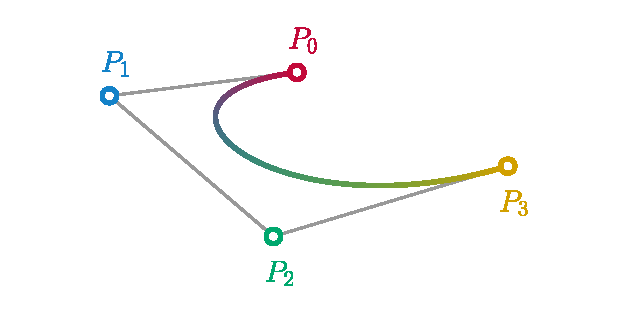
\includegraphics[width=\linewidth]{figures/3_1_cubic_polynomial_bezier_curve.pdf}\\[0.5cm]
            \visible<2->
            {
            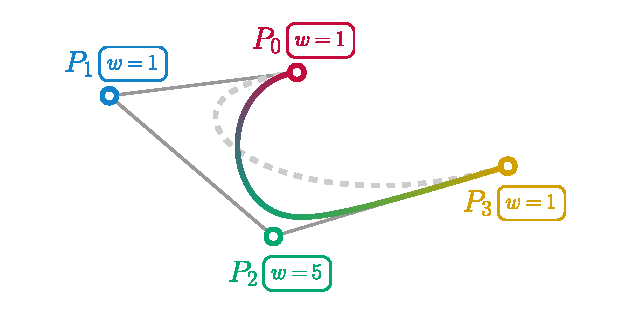
\includegraphics[width=\linewidth]{figures/3_2_cubic_rational_bezier_curve.pdf}\\[0.5cm]
            }
        \end{minipage}

    \end{columns}
\end{frame}
%%%%%%%%%%%%%%%%%%%%%%%%%%%%%%%%%%%%%%%%%%%%%%%%%%%%%%%%%%%%%%%%%%%%%%%%%%%%%%%%%%%%%%%%%%%%%%%%%


%%%%%%%%%%%%%%%%%%%%%%%%%%%%%%%%%%%%%%%%%%%%%%%%%%%%%%%%%%%%%%%%%%%%%%%%%%%%%%%%%%%%%%%%%%%%%%%%%
\begin{frame}[t]{\textbf{PGA} : Plane-based Geometric Algebra}
            \[\mathbf{e}_0^2 = 0 \quad \mathbf{e}_1^2 = \ldots = \mathbf{e}_n^2 = 1 \]
            \[\mathbf{e}_i\cdot \mathbf{e}_j = 0, i\neq j\]
        \begin{align*}
            \textbf{Hyperplanes : } \mathbf{a} = & a_0\mathbf{e}_0 + a_1\mathbf{e}_1 + \cdots + a_n\mathbf{e}_n \\
            \textbf{Points : } \mathbf{P} = (&w\mathbf{e}_0 + x_1\mathbf{e}_1 + \cdots + x_n\mathbf{e}_n)^\star
        \end{align*}

        \vspace{0.5cm}
        \visible<2->
        {
        In 2D: hyperplanes $\rightarrow$ \textbf{Lines} : $\mathbf{L} = c\mathbf{e}_0 + a\mathbf{e}_1 + b\mathbf{e}_2$
        

        \begin{center}
        \only<2>
        {
            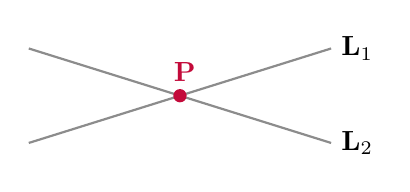
\begin{tikzpicture}[scale=1.2]
                \draw[thick, black!45] (-1.6,-0.5) -- (1.6,0.5)
                    node[right, black] {$\mathbf{L}_1$};
                \draw[thick, black!45] (-1.6,0.5) -- (1.6,-0.5)
                    node[right, black] {$\mathbf{L}_2$};
                \fill[PGAred] (0,0) circle (2pt);
                \node[above, PGAred] at (0.05,0.05) {$\mathbf{P}$};
            \end{tikzpicture}
        }
        \only<3>
        {
            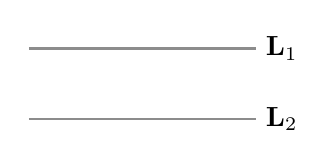
\begin{tikzpicture}[scale=0.9]
                \draw[thick, black!45] (-1.6,0.5) -- (1.6,0.5)
                    node[right, black] {$\mathbf{L}_1$};
                \draw[thick, black!45] (-1.6,-0.5) -- (1.6,-0.5)
                    node[right, black] {$\mathbf{L}_2$};
            \end{tikzpicture}
         }
            \[
                \mathbf{P} = (w\mathbf{e}_0 + x\mathbf{e}_1 + y\mathbf{e}_2)^\star
            \]
        \end{center}
        }
\end{frame}
%%%%%%%%%%%%%%%%%%%%%%%%%%%%%%%%%%%%%%%%%%%%%%%%%%%%%%%%%%%%%%%%%%%%%%%%%%%%%%%%%%%%%%%%%%%%%%%%%

%%%%%%%%%%%%%%%%%%%%%%%%%%%%%%%%%%%%%%%%%%%%%%%%%%%%%%%%%%%%%%%%%%%%%%%%%%%%%%%%%%%%%%%%%%%%%%%%%
\begin{frame}[t]{PGA Finite and Ideal}
    \setlength{\columnsep}{20pt}

    \begin{columns}[T,onlytextwidth]
        \begin{column}{0.5\textwidth}
            \centering
            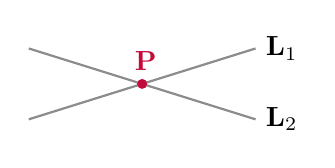
\begin{tikzpicture}[scale=0.9]
                \draw[thick, black!45] (-1.6,-0.5) -- (1.6,0.5)
                    node[right, black] {$\mathbf{L}_1$};
                \draw[thick, black!45] (-1.6,0.5) -- (1.6,-0.5)
                    node[right, black] {$\mathbf{L}_2$};
                \fill[PGAred] (0,0) circle (2pt);
                \node[above, PGAred] at (0.05,0.05) {$\mathbf{P}$};
            \end{tikzpicture}
            
            \alert{\textbf{Finite Point}}
            \visible<2->
            {
            \[
                \textcolor{PGAred}{\mathbf{P}} = (w\mathbf{e}_0 + x\mathbf{e}_1 + y\mathbf{e}_2)^\star
            \]
            }
            \visible<3->
            {
            \[
                \|\textcolor{PGAred}{\mathbf{P}}\| = \|\textcolor{PGAred}{\mathbf{P}}\|_f = \sqrt{\textcolor{PGAred}{\mathbf{P}}\,\widetilde{\textcolor{PGAred}{\mathbf{P}}}} = |w|
            \]
            }
            
        
        \end{column}
        
        
        \begin{column}{0.5\textwidth}
            \centering
            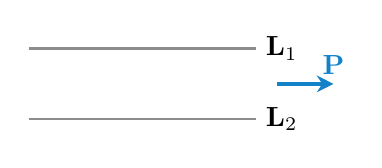
\begin{tikzpicture}[scale=0.9]
                \draw[thick, black!45] (-1.6,0.5) -- (1.6,0.5)
                    node[right, black] {$\mathbf{L}_1$};
                \draw[thick, black!45] (-1.6,-0.5) -- (1.6,-0.5)
                    node[right, black] {$\mathbf{L}_2$};
                \draw[->, PGAblue, line width=1.2pt, -{Stealth[length=6pt, width=6pt]}] (1.9,0) -- (2.7,0);
                \node[above, PGAblue] at (2.7,0) {$\mathbf{P}$};
            \end{tikzpicture}
            
            \alert{\textbf{Ideal Point}}
            \visible<2->{\[
                \textcolor{PGAblue}{\mathbf{P}} = (\textcolor{gray}{0 \mathbf{e}_0 +} x\mathbf{e}_1 + y\mathbf{e}_2)^\star
            \]}
            \visible<3->{\[
                \|\textcolor{PGAblue}{\mathbf{P}}\| = \|\textcolor{PGAblue}{\mathbf{P}}\|_\infty = \|\textcolor{PGAblue}{\mathbf{P}}^\star\|_f = \sqrt{x^2+y^2}
            \]}
            
        \end{column}
    \end{columns}

    
    \vspace{0.5cm}
    \visible<4->
    {
    \textbf{\alert{Adaptative normalization}} \textcolor{gray}{(coordinate-free)}: \[\hat{A} = \displaystyle\frac{A}{\|A\|}\]
    }
\end{frame}
%%%%%%%%%%%%%%%%%%%%%%%%%%%%%%%%%%%%%%%%%%%%%%%%%%%%%%%%%%%%%%%%%%%%%%%%%%%%%%%%%%%%%%%%%%%%%%%%%

% ============================================================================
% BLOCK C — BÉZIER IN PGA: UNIFICATION
% ============================================================================

%%%%%%%%%%%%%%%%%%%%%%%%%%%%%%%%%%%%%%%%%%%%%%%%%%%%%%%%%%%%%%%%%%%%%%%%%%%%%%%%%%%%%%%%%%%%%%%%%
\section{Bézier Curves in PGA}
%%%%%%%%%%%%%%%%%%%%%%%%%%%%%%%%%%%%%%%%%%%%%%%%%%%%%%%%%%%%%%%%%%%%%%%%%%%%%%%%%%%%%%%%%%%%%%%%%


%%%%%%%%%%%%%%%%%%%%%%%%%%%%%%%%%%%%%%%%%%%%%%%%%%%%%%%%%%%%%%%%%%%%%%%%%%%%%%%%%%%%%%%%%%%%%%%%%
\begin{frame}[t]{Projective Bézier Curves in PGA}
    \setlength{\columnsep}{20pt}

        % The \alert{\textbf{PGA Bézier curve}}:
        % Weights $\lambda_i$ are separate from the homogeneous coordinate $w$.
        \begin{align*}
            % Dans le préambule : \usepackage{mathtools}
            \text{The \alert{\textbf{PGA Bézier curve}}} \qquad
            \Aboxed{\mathbf{P}(t) &= \sum_{i=0}^{d} B_i^d(t)\, \lambda_i\, \hat{\mathbf{P}}_i} \\
            \visible<2->{&= \sum_{i=0}^{d} B_i^d(t)\, \lambda_i\, (\mathbf{e}_0 + x \mathbf{e}_1 + y \mathbf{e}_2)^\star \\
            &= \underbrace{\sum_{i=0}^{d} B_i^d(t)\, \lambda_i \mathbf{e}_0^\star}_{\displaystyle w \mathbf{e}_0^\star} + \sum_{i=0}^{d} B_i^d(t)\, \lambda_i (x \mathbf{e}_1 + y \mathbf{e}_2)^\star}
        \end{align*}

        \vspace{0.25cm}
        \visible<3->
        {
        \textbf{Projective normalization} (coordinate-free):
        \[
            \hat{\mathbf{P}}(t) = \frac{\mathbf{P}(t)}{\|\mathbf{P}(t)\|}
            = \frac{\sum_{i=0}^{d} B_i^d(t)\, \lambda_i ( \mathbf{e}_0 + x \mathbf{e}_1 + y \mathbf{e}_2)^\star}{| \sum_{i=0}^{d} B_i^d(t)\, \lambda_i |}
            \underbrace{=}_{\lambda_i > 0} \frac{\sum_{i=0}^{d} B_i^d(t)\, \lambda_i \mathbf{P}_i}{\sum_{i=0}^{d} B_i^d(t)\, \lambda_i}
        \]
        }
        
       % For finite points, $\|\mathbf{P}(t)\|$ is already encoded in $\mathbf{P}(t)$: \alert{no explicit division required}.


        % \begin{minipage}[c][0.8\textheight][c]{\linewidth}
        %     \centering
        %     \begin{block}{What we gain}
        %         \begin{itemize}\setlength\itemsep{0.2em}
        %             \item Weights $\lambda_i$ independent of point representation
        %             \item All operations stay in projective form
        %             \item Recovers classical rational Bézier when $\lambda_i > 0$
        %             %\item \alert{Same equation} extends to negative weights, ideal points, lines, planes, versors
        %         \end{itemize}
        %     \end{block}
        % \end{minipage}

\end{frame}
%%%%%%%%%%%%%%%%%%%%%%%%%%%%%%%%%%%%%%%%%%%%%%%%%%%%%%%%%%%%%%%%%%%%%%%%%%%%%%%%%%%%%%%%%%%%%%%%%


% ============================================================================
% BLOCK D — NEGATIVE WEIGHTS & COMPLEMENTARY CURVE
% ============================================================================

%%%%%%%%%%%%%%%%%%%%%%%%%%%%%%%%%%%%%%%%%%%%%%%%%%%%%%%%%%%%%%%%%%%%%%%%%%%%%%%%%%%%%%%%%%%%%%%%%
\begin{frame}[t]{Negative Weights: $\lambda_i \in \mathbb{R}^*$}
    \setlength{\columnsep}{20pt}
    % \[
    %     \hat{\mathbf{P}}(t) = \displaystyle\frac{\mathbf{P}(t)}{\|\mathbf{P}(t)\|} \quad \text{ with } \quad \|\mathbf{P}(t)\| = \begin{cases} 
    %     \|\mathbf{P}(t)\|_f & \text{if } \mathbf{P}(t) \text{ is finite,} \\
    %     \|\mathbf{P}(t)\|_\infty & \text{if } \mathbf{P}(t) \text{ is ideal}
    % \end{cases}
    % \]
    If $\sum_i B_i^d(t) \lambda_i =0 \leftrightarrow w(t)=0$ for some $t$ \visible<2->{: $\mathbf{P}(t)$ is just an \textbf{\alert{ideal point}} !} 

        %     \|\mathbf{P}(t)\|_f &= \sum_i B_i^d(t) \lambda_i    \\
        % \|\mathbf{P}(t)\|_\infty  &= \sqrt{\big(\sum_{i=0}^{d} B_i^d(t)\, \lambda_i \, x \big)^2 +\big(\sum_{i=0}^{d} B_i^d(t)\, \lambda_i \,y \big)^2 }
    
    \begin{columns}[T]
        

        \column{0.48\textwidth}

        
        % with $\|\mathbf{P}(t)\| = \sum_i B_i^d(t)\, \lambda_i$
       \vspace{0.8cm}

        \visible<3->
        {
        \[
        \hat{\mathbf{P}}(t) = \displaystyle\frac{\mathbf{P}(t)}{\|\mathbf{P}(t)\|} \quad
        \]
        \[
            \|\mathbf{P}(t)\| = \begin{cases} 
            \|\mathbf{P}(t)\|_f & \text{if } \mathbf{P}(t) \text{ is finite,} \\
            \|\mathbf{P}(t)\|_\infty & \text{if } \mathbf{P}(t) \text{ is ideal}
        \end{cases}
        \]
        }
        
           
        % If $\sum_i B_i^d(t) \lambda_i =0$ for some $t$:
        % \begin{itemize}\setlength\itemsep{0.15em}
        %     % \item Classically: undefined singularity
        %     \item In PGA: $\mathbf{P}(t)$ becomes an \alert{ideal point}
        %     \item General norm switches to $\|\cdot\|_\infty$
        %     %normalization stays well-defined
        % \end{itemize}

        \vspace{0.8cm}
        \visible<5->
        {
        \textbf{Geometric meaning:}
        \begin{itemize}\setlength\itemsep{0.15em}
            %\item Positive weight $\to$ attraction toward~$\hat{\mathbf{P}}_i$
            \item Negative weight $\to$ \alert{repulsion}
            \item Singularity $\to$ asymptotic direction %encoded directly in $\mathbf{P}(t)$
        \end{itemize}
        }
        
        \column{0.52\textwidth}

        \visible<4->
        {
        \begin{minipage}[c][0.8\textheight][c]{\linewidth}
            \centering
            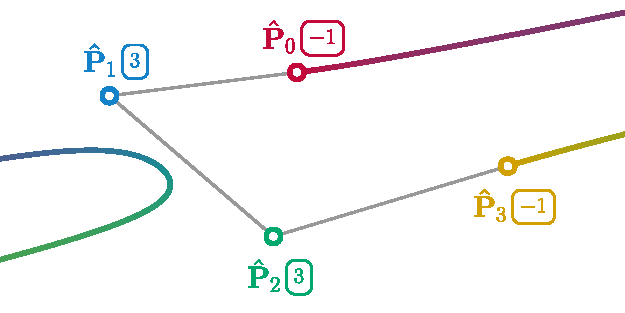
\includegraphics[width=\linewidth]{figures/4_2_cubic_rational_bezier_curve.pdf}\\[0.15cm]
        \end{minipage}
        }
        
    \end{columns}
\end{frame}
%%%%%%%%%%%%%%%%%%%%%%%%%%%%%%%%%%%%%%%%%%%%%%%%%%%%%%%%%%%%%%%%%%%%%%%%%%%%%%%%%%%%%%%%%%%%%%%%%


%%%%%%%%%%%%%%%%%%%%%%%%%%%%%%%%%%%%%%%%%%%%%%%%%%%%%%%%%%%%%%%%%%%%%%%%%%%%%%%%%%%%%%%%%%%%%%%%%
\begin{frame}[t]{Complementary Curve Section}
    \setlength{\columnsep}{20pt}
    \begin{columns}[T]

        \column{0.48\textwidth}
        \vspace{1.0cm}
        \textbf{Endpoint tangents:}
        \begin{align*}
            \mathbf{P}'(0) &\propto \tfrac{\lambda_1}{\lambda_0}(\mathbf{P}_1 - \mathbf{P}_0) \\
            \mathbf{P}'(1) &\propto \tfrac{\lambda_{d-1}}{\lambda_d}(\mathbf{P}_d - \mathbf{P}_{d-1})
        \end{align*}

        \vspace{1.0cm}
        \visible<2->
        {
        \textbf{Flip endpoint weight signs}\\ %\ \ $\lambda_0 \to -\lambda_0$,\ $\lambda_d \to -\lambda_d$ 
        $\Rightarrow$ tangent directions reverse at endpoints
        }

        % \vspace{0.2cm}
        % Same endpoints, opposite tangents: the curve traces the \alert{complementary section} of the same underlying algebraic curve.

        \column{0.52\textwidth}
        \vspace{0.66cm}
        \begin{minipage}[c][0.8\textheight][c]{\linewidth}
            \centering
            \only<1>
            {
            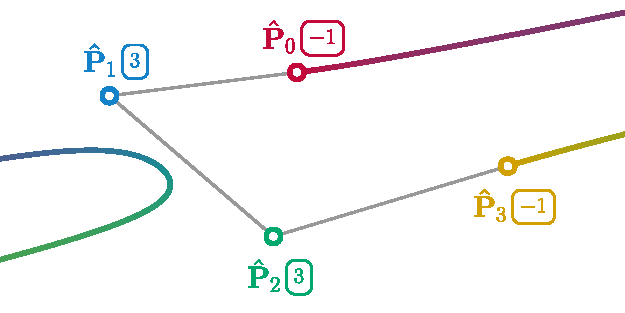
\includegraphics[width=\linewidth]
            {figures/4_2_cubic_rational_bezier_curve.pdf}\\[0.15cm]
            } \only<2>{
            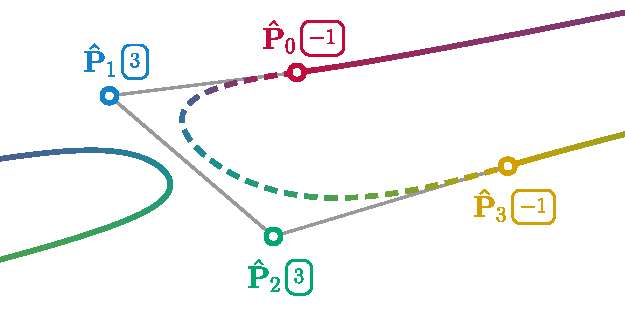
\includegraphics[width=\linewidth]{figures/4_2_cubic_rational_bezier_curve_complementary.pdf}\\[0.15cm]
            }
        \end{minipage}

    \end{columns}
\end{frame}
%%%%%%%%%%%%%%%%%%%%%%%%%%%%%%%%%%%%%%%%%%%%%%%%%%%%%%%%%%%%%%%%%%%%%%%%%%%%%%%%%%%%%%%%%%%%%%%%%


% ============================================================================
% BLOCK E — CONICS & IDEAL POINTS
% ============================================================================

%%%%%%%%%%%%%%%%%%%%%%%%%%%%%%%%%%%%%%%%%%%%%%%%%%%%%%%%%%%%%%%%%%%%%%%%%%%%%%%%%%%%%%%%%%%%%%%%%
\begin{frame}[t]{Conics as Quadratic Rational Bézier}


        % Quadratic denominator $Q(t) = \sum B_i^2(t)\lambda_i$. Real roots $\Leftrightarrow$ curve reaches infinity.
% \visible<1>{
%         \[
%         \mathbf{P}(t) = \frac{B_0(t) \lambda_0 \mathbf{P}_0 + B_1(t) \lambda_1\mathbf{P}_1 + B_2(t) \lambda_2 \mathbf{P}_2}{B_0(t) \lambda_0 + B_1(t) \lambda_1 + B_2(t) \lambda_2}
%         \]
%         }%


        \[
        \mathbf{P}(t) = \frac{B_0(t) \lambda_0 \mathbf{P}_0 + B_1(t) \lambda_1\mathbf{P}_1 + B_2(t) \lambda_2 \mathbf{P}_2}{B_0(t) \lambda_0 + B_1(t) \lambda_1 + B_2(t) \lambda_2}
        \]

        \visible<2->
        {
        \[
        Q(t) = (1-t)^2 \lambda_0 + 2t(1-t) \lambda_1 + t^2 \lambda_2
        \qquad \quad \Delta = 4(\lambda_1^2 - \lambda_0 \lambda_2)
        \]
        }

        
        % \vspace{0.15cm}
        % Discriminant: $\Delta = 4(\lambda_1^2 - \lambda_0 \lambda_2)$

        % \vspace{0.1cm}
        % \textbf{Projective trichotomy:}
        % \begin{itemize}\setlength\itemsep{0.15em}
        %     \item $\Delta < 0$: \alert{ellipse} (no real root)
        %     \item $\Delta = 0$: \alert{parabola} (tangent to $\infty$)
        %     \item $\Delta > 0$: \alert{hyperbola} (crosses $\infty$ twice)
        % \end{itemize}

        % \vspace{0.1cm}
        % Sign flips preserve $\Delta$: same conic, complementary section.
        \visible<3->
        {
        \begin{center}
        \hspace{-1.3cm}
        \begin{tabular}{ccc}
        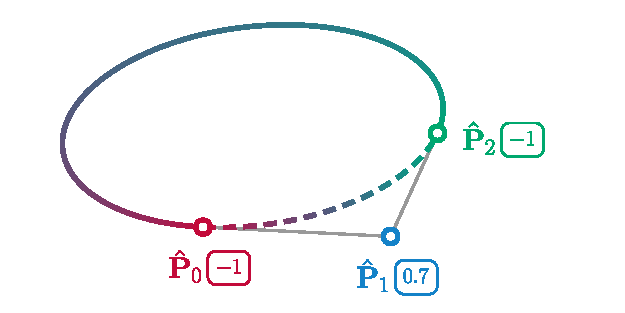
\includegraphics[width=0.33\linewidth]{figures/4_2_1_quadratic_rational_bezier_ellipse.pdf} 
        &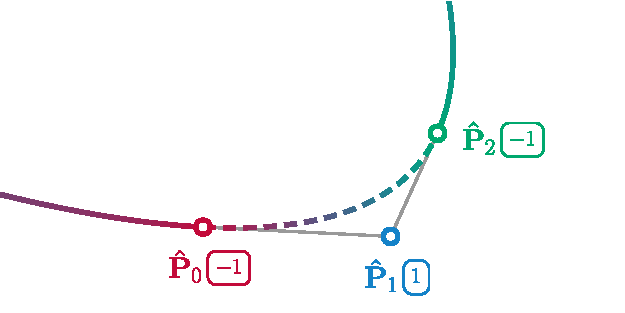
\includegraphics[width=0.33\linewidth]{figures/4_2_1_quadratic_rational_bezier_parabola.pdf} 
        &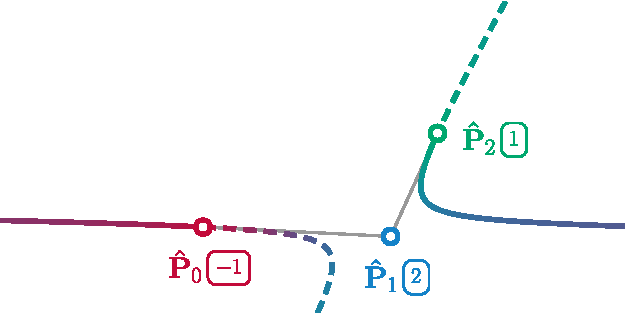
\includegraphics[width=0.33\linewidth]{figures/4_2_1_quadratic_rational_bezier_hyperbola.pdf}\\
        \textbf{\alert{Ellipse}}
        & \textbf{\alert{Parabola}}
        & \textbf{\alert{Hyperbola}} \\
        $\Delta < 0$
        & $\Delta = 0$
        & $\Delta > 0$
        \end{tabular}
        \end{center}
        % \begin{minipage}[c][0.8\textheight][c]{\linewidth}
        %     \centering
        %     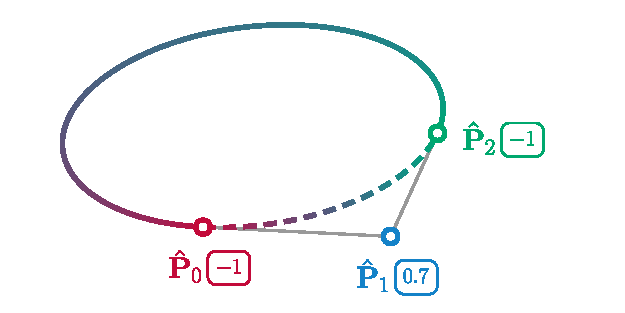
\includegraphics[width=0.7\linewidth]{figures/4_2_1_quadratic_rational_bezier_ellipse.pdf}\\[0.02cm]
        %     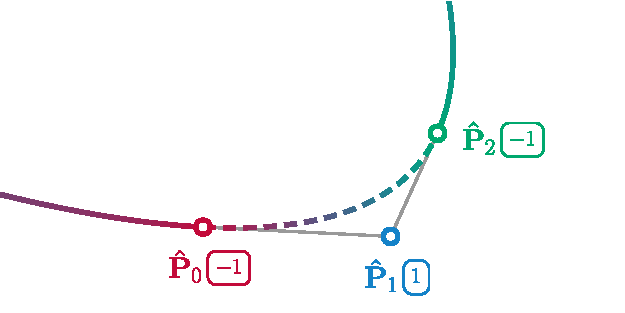
\includegraphics[width=0.7\linewidth]{figures/4_2_1_quadratic_rational_bezier_parabola.pdf}\\[0.02cm]
        %     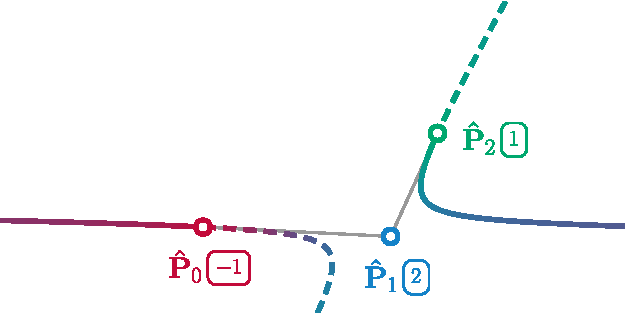
\includegraphics[width=0.7\linewidth]{figures/4_2_1_quadratic_rational_bezier_hyperbola.pdf}
        % \end{minipage}
        }

\end{frame}
%%%%%%%%%%%%%%%%%%%%%%%%%%%%%%%%%%%%%%%%%%%%%%%%%%%%%%%%%%%%%%%%%%%%%%%%%%%%%%%%%%%%%%%%%%%%%%%%%


%%%%%%%%%%%%%%%%%%%%%%%%%%%%%%%%%%%%%%%%%%%%%%%%%%%%%%%%%%%%%%%%%%%%%%%%%%%%%%%%%%%%%%%%%%%%%%%%%
\begin{frame}[t]{Finite and Ideal Control Points}

     \[
        \mathbf{P}(t) = \sum_{i=0}^{d} B_i^d(t)\, \lambda_i\, \hat{\mathbf{P}}_i
        \qquad \quad
        \visible<2->{
        \hat{\mathbf{P}}_i = \begin{dcases} 
           \frac{w \mathbf{e}_0 + x \mathbf{e}_1 + y \mathbf{e}_2}{|w|} & \text{if \alert{finite},} \\[6pt]
           \frac{\mathbf{e}_1 + y \mathbf{e}_2}{\sqrt{x^2+y^2}} & \text{if \alert{ideal}}
        \end{dcases}}
    \]

    \begin{center}
        \begin{tabular}{cc}
        \visible<3->{
        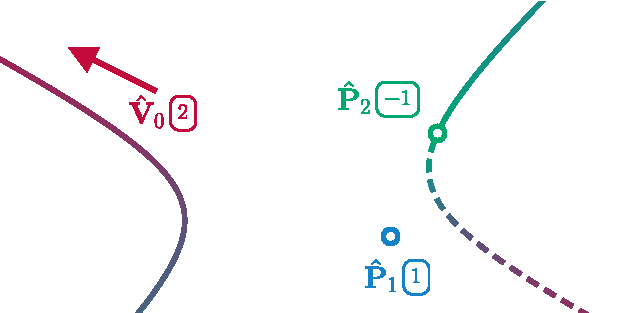
\includegraphics[width=0.4\linewidth]{figures/4_3_quadratic_rational_bezier_point_vector_endpoint.pdf}}
        &\visible<4->{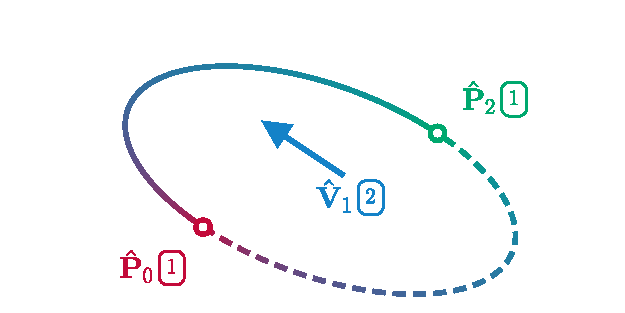
\includegraphics[width=0.4\linewidth]{figures/4_3_quadratic_rational_bezier_point_vector_transition.pdf}} \\
        \visible<3->{
        \textbf{\alert{Endpoint ideal}}}
        & \visible<4->{\textbf{\alert{Interior ideal}}} \\
        \visible<3->{
        asymptotic direction}
        & \visible<4->{directional control}
        \end{tabular}
    \end{center}
\end{frame}
%%%%%%%%%%%%%%%%%%%%%%%%%%%%%%%%%%%%%%%%%%%%%%%%%%%%%%%%%%%%%%%%%%%%%%%%%%%%%%%%%%%%%%%%%%%%%%%%%


%%%%%%%%%%%%%%%%%%%%%%%%%%%%%%%%%%%%%%%%%%%%%%%%%%%%%%%%%%%%%%%%%%%%%%%%%%%%%%%%%%%%%%%%%%%%%%%%%
\begin{frame}[t]{Ideal Control Points}

     \[
        \mathbf{P}(t) = \sum_{i=0}^{d} B_i^d(t)\, \lambda_i\, \hat{\mathbf{P}}_i
        \qquad \quad
        \hat{\mathbf{P}}_i =  \displaystyle \frac{x \mathbf{e}_1 + y \mathbf{e}_2}{\sqrt{x^2+y^2}}
     \]
    \vspace{0.5cm}
    \begin{center}
        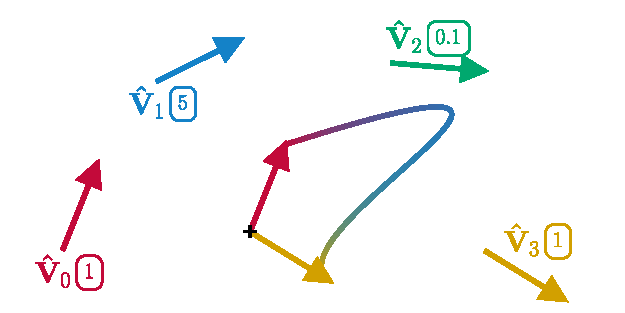
\includegraphics[width=0.5\linewidth]{figures/4_4_cubic_ideal_points_aligned_vectors.pdf}
    \end{center}
\end{frame}
%%%%%%%%%%%%%%%%%%%%%%%%%%%%%%%%%%%%%%%%%%%%%%%%%%%%%%%%%%%%%%%%%%%%%%%%%%%%%%%%%%%%%%%%%%%%%%%%%


% ============================================================================
% BLOCK F — GENERALIZATION: OBJECTS & VERSORS
% ============================================================================

%%%%%%%%%%%%%%%%%%%%%%%%%%%%%%%%%%%%%%%%%%%%%%%%%%%%%%%%%%%%%%%%%%%%%%%%%%%%%%%%%%%%%%%%%%%%%%%%%
\section{Generalization}
%%%%%%%%%%%%%%%%%%%%%%%%%%%%%%%%%%%%%%%%%%%%%%%%%%%%%%%%%%%%%%%%%%%%%%%%%%%%%%%%%%%%%%%%%%%%%%%%%


%%%%%%%%%%%%%%%%%%%%%%%%%%%%%%%%%%%%%%%%%%%%%%%%%%%%%%%%%%%%%%%%%%%%%%%%%%%%%%%%%%%%%%%%%%%%%%%%%
\begin{frame}[t]{Bézier of Lines}
        \[
         \mathbf{L} = c\mathbf{e}_0 + a\mathbf{e}_1 + b\mathbf{e}_2 \qquad   \hat{\mathbf{L}} = \frac{\mathbf{L}}{\|\mathbf{L}\|} 
        \]       \qquad 
        \[
            \mathbf{L}(t) = \sum_{i=0}^{d} B_i^d(t)\, \lambda_i\, \hat{\mathbf{L}}_i
        \]
        \vspace{0.5cm}

        \visible<2->
        {
        \begin{center}
                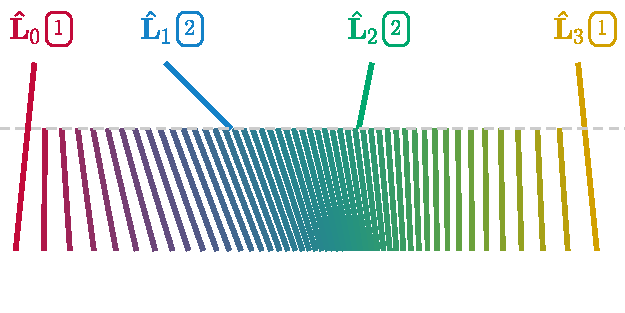
\includegraphics[width=0.5\linewidth]{figures/5_1_cubic_bezier_curve_lines.pdf}
        \end{center}
        }

\end{frame}
%%%%%%%%%%%%%%%%%%%%%%%%%%%%%%%%%%%%%%%%%%%%%%%%%%%%%%%%%%%%%%%%%%%%%%%%%%%%%%%%%%%%%%%%%%%%%%%%%


%%%%%%%%%%%%%%%%%%%%%%%%%%%%%%%%%%%%%%%%%%%%%%%%%%%%%%%%%%%%%%%%%%%%%%%%%%%%%%%%%%%%%%%%%%%%%%%%%
\begin{frame}[t]{Bézier of Planes}
        \[
         \pmb{\Pi} = a_0\mathbf{e}_0 + a_1\mathbf{e}_1 + a_2\mathbf{e}_2 + a_3\mathbf{e}_3 \qquad   \hat{\pmb{\Pi}} = \frac{\pmb{\Pi}}{\|\pmb{\Pi}\|} 
        \] 
        \[
            \pmb{\Pi}(t) = \sum_{i=0}^{d} B_i^d(t)\, \lambda_i\, \hat{\pmb{\Pi}}_i
        \]
        \vspace{-1.0cm}
        % Same blending equation, applied to \alert{lines}:
        % Bernstein \alert{partition of unity} preserves grade: the blend of grade-1 blades is still a line.
        % Ideal lines ($\mathbf{L} = \mathbf{e}_0$) handled uniformly by the adaptive norm.
        \visible<2->
        {
        \begin{center}
                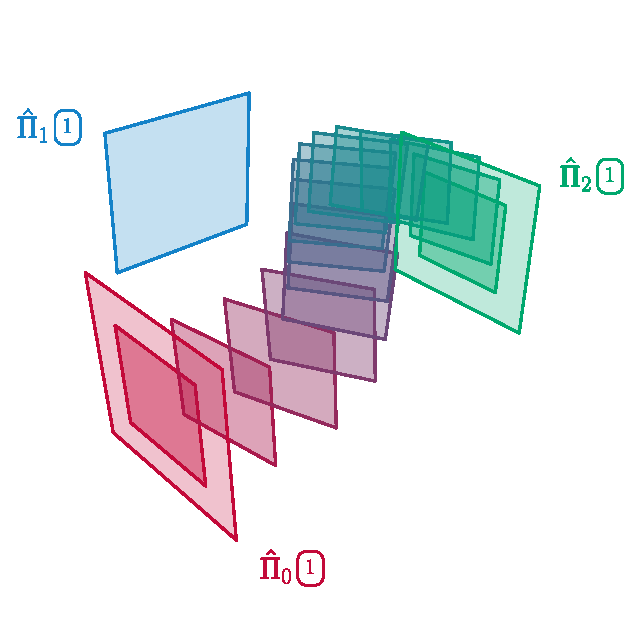
\includegraphics[width=0.4\linewidth]{figures/planes_bezier.pdf}
        \end{center}
        }
\end{frame}
%%%%%%%%%%%%%%%%%%%%%%%%%%%%%%%%%%%%%%%%%%%%%%%%%%%%%%%%%%%%%%%%%%%%%%%%%%%%%%%%%%%%%%%%%%%%%%%%%



%%%%%%%%%%%%%%%%%%%%%%%%%%%%%%%%%%%%%%%%%%%%%%%%%%%%%%%%%%%%%%%%%%%%%%%%%%%%%%%%%%%%%%%%%%%%%%%%%
\begin{frame}[t]{Bézier of Hyperplanes}
    \setlength{\columnsep}{20pt}
    \begin{columns}[T]
        \column{0.48\textwidth}
        \vspace{1.0cm}
        In $n$-d PGA : Bézier curve of \alert{hyperplanes}:
        \[
         \mathbf{h} = a_0\mathbf{e}_0 + a_1\mathbf{e}_1 + \ldots + a_n\mathbf{e}_n \qquad   \hat{\mathbf{h}} = \frac{\mathbf{h}}{\|\mathbf{h}\|} 
        \] 
        \[
            \mathbf{h}(t) = \sum_{i=0}^{d} B_i^d(t)\, \lambda_i\, \hat{\mathbf{h}}_i
        \]

        \vspace{0.15cm}
        % \textbf{Take-away:} one equation, all geometric objects of PGA (points, lines, planes, 3D lines, $\ldots$).

        \column{0.52\textwidth}

        \begin{minipage}[c][0.8\textheight][c]{\linewidth}
            \centering
            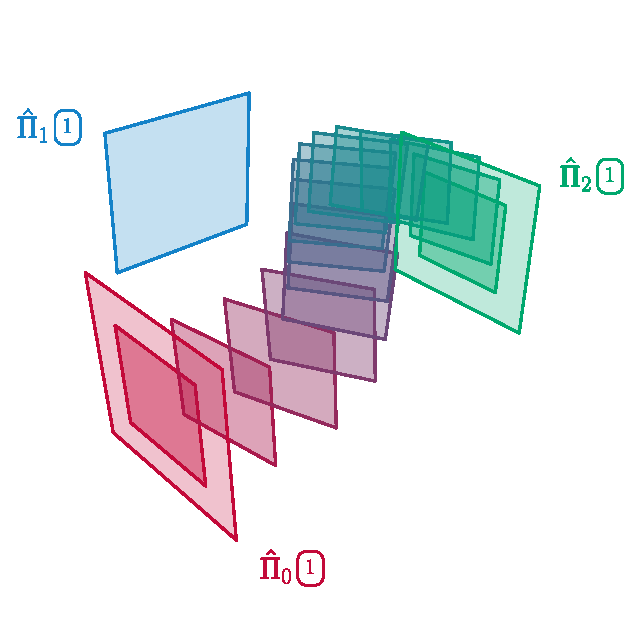
\includegraphics[width=0.7\linewidth]{figures/planes_bezier.pdf}\\[0.1cm]
        \end{minipage}

    \end{columns}
\end{frame}
%%%%%%%%%%%%%%%%%%%%%%%%%%%%%%%%%%%%%%%%%%%%%%%%%%%%%%%%%%%%%%%%%%%%%%%%%%%%%%%%%%%%%%%%%%%%%%%%%


%%%%%%%%%%%%%%%%%%%%%%%%%%%%%%%%%%%%%%%%%%%%%%%%%%%%%%%%%%%%%%%%%%%%%%%%%%%%%%%%%%%%%%%%%%%%%%%%%
\begin{frame}[t]{Bézier of Versors: Smooth Rigid Motions}
    \setlength{\columnsep}{20pt}
    \begin{columns}[T]

        \column{0.48\textwidth}
        \vspace{1.5cm}
        Versors encode \alert{rigid transformations} :
         $$\mathbf{X}(t) = \hat{V}(t)\, \mathbf{X}\, \widetilde{\hat{V}}(t)$$
        
        %; \textbf{motors} combine rotation $+$ translation.

        \vspace{0.4cm}
        \visible<2->
        {
        %Same blending, then renormalize:
        Bezier of \alert{Versors} :
        \[
            V(t) = \sum_{i=0}^{d} B_i^d(t)\, \lambda_i \hat{V}_i 
        \]
        }
        % \[
        %     \hat{V}(t) = \frac{V(t)}{\|V(t)\|}
        % \]

       % \vspace{0.15cm}
      %  Apply via sandwich: $\mathbf{X}(t) = \hat{V}(t)\, \mathbf{X}\, \widetilde{\hat{V}(t)}$

       % \vspace{0.15cm}
       % \alert{Smooth family of rigid motions} for geometric animation. Linear blend, not geodesic (ScLERP is future work).

        \column{0.52\textwidth}
        \vspace{1.5cm}
        \visible<2->
        {
        \begin{center}
            \centering
            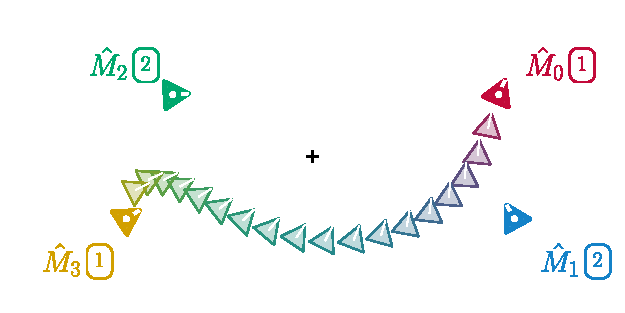
\includegraphics[width=1.0\linewidth]{figures/bezier_motors.pdf}\\[0.1cm]
        \end{center}
        }
    \end{columns}
\end{frame}
%%%%%%%%%%%%%%%%%%%%%%%%%%%%%%%%%%%%%%%%%%%%%%%%%%%%%%%%%%%%%%%%%%%%%%%%%%%%%%%%%%%%%%%%%%%%%%%%%


% ============================================================================
% BLOCK G — RESULTS GALLERY & CONCLUSION
% ============================================================================

%%%%%%%%%%%%%%%%%%%%%%%%%%%%%%%%%%%%%%%%%%%%%%%%%%%%%%%%%%%%%%%%%%%%%%%%%%%%%%%%%%%%%%%%%%%%%%%%%
\begin{frame}[t]{Conclusion 1/2}
    \setlength{\columnsep}{15pt}
    \begin{columns}[T]

        \column{0.45\textwidth}
            $$\displaystyle \mathbf{X}(t) = \sum_{i=0}^{d} B_i^d(t)\, \lambda_i\, \hat{\mathbf{X}}_i$$

        \vspace{0.8cm}
\textbf{One Equation, many Curves :}
        \begin{itemize}\setlength\itemsep{0.15em}
            \item Points \textcolor{gray}{(finite + ideal)}
            \item Negative weights :
               \begin{itemize}
                   \item complementary sections
                   \item conics
               \end{itemize}
            \item Lines, planes, hyperplanes
            \item Versors : rigid-motion animation
        \end{itemize}

        \column{0.55\textwidth}

        \begin{minipage}[c][0.8\textheight][c]{\linewidth}
            \centering
            \begin{tabular}{@{}cc@{}}
                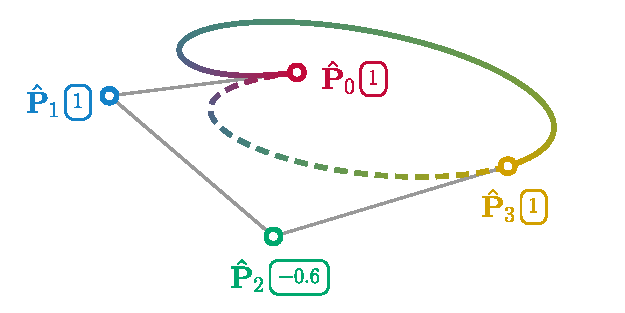
\includegraphics[width=0.42\linewidth]{figures/4_2_cubic_rational_bezier_curve_negative_weight_repulse.pdf} &
                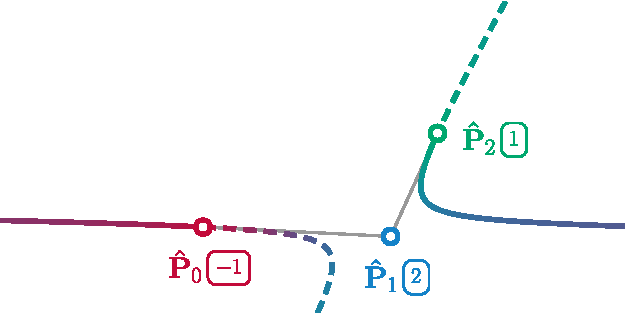
\includegraphics[width=0.42\linewidth]{figures/4_2_1_quadratic_rational_bezier_hyperbola.pdf} \\[0.02cm]
                {\small Negative weight} & {\small Hyperbola} \\ ~\\ ~\\[0.05cm]
                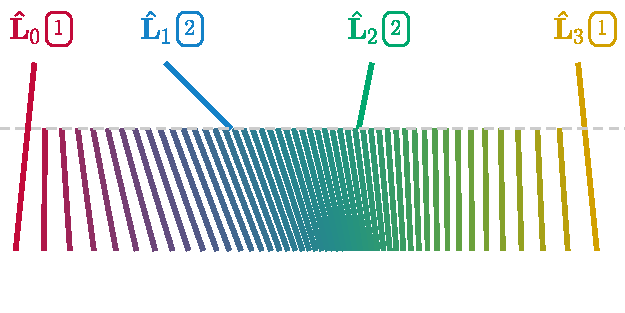
\includegraphics[width=0.42\linewidth]{figures/5_1_cubic_bezier_curve_lines.pdf} &
                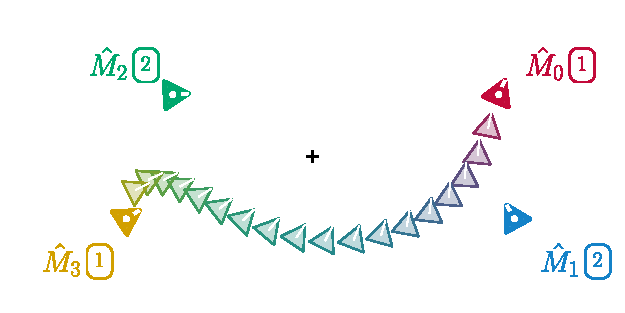
\includegraphics[width=0.42\linewidth]{figures/bezier_motors.pdf} \\[0.02cm]
                {\small Bézier of lines} & {\small Bézier of motors}
            \end{tabular}
        \end{minipage}

    \end{columns}
\end{frame}
%%%%%%%%%%%%%%%%%%%%%%%%%%%%%%%%%%%%%%%%%%%%%%%%%%%%%%%%%%%%%%%%%%%%%%%%%%%%%%%%%%%%%%%%%%%%%%%%%


%%%%%%%%%%%%%%%%%%%%%%%%%%%%%%%%%%%%%%%%%%%%%%%%%%%%%%%%%%%%%%%%%%%%%%%%%%%%%%%%%%%%%%%%%%%%%%%%%
\begin{frame}[t]{Conclusion 2/2}
    % \begin{block}{Contributions}
    %     Bézier curves reformulated in PGA, unifying:
    %     \begin{itemize}\setlength\itemsep{0.15em}
    %         \item Rational Bézier with arbitrary real weights (including negative)
    %         \item Finite and ideal control points
    %         \item Geometric objects of any grade (points, lines, planes, hyperplanes)
    %         \item Versors $\to$ smooth Bézier curves of rigid motions
    %     \end{itemize}
    % \end{block}

    % \vspace{0.1cm}
    \begin{block}{Source code}
    \alert{Interactive notebooks:} {\small \url{https://eharquin.github.io/pga-bezier/}}
    \vspace{-0.3cm}
    \begin{center}  
    {\setlength{\fboxsep}{0pt}\setlength{\fboxrule}{0.4pt}\fbox{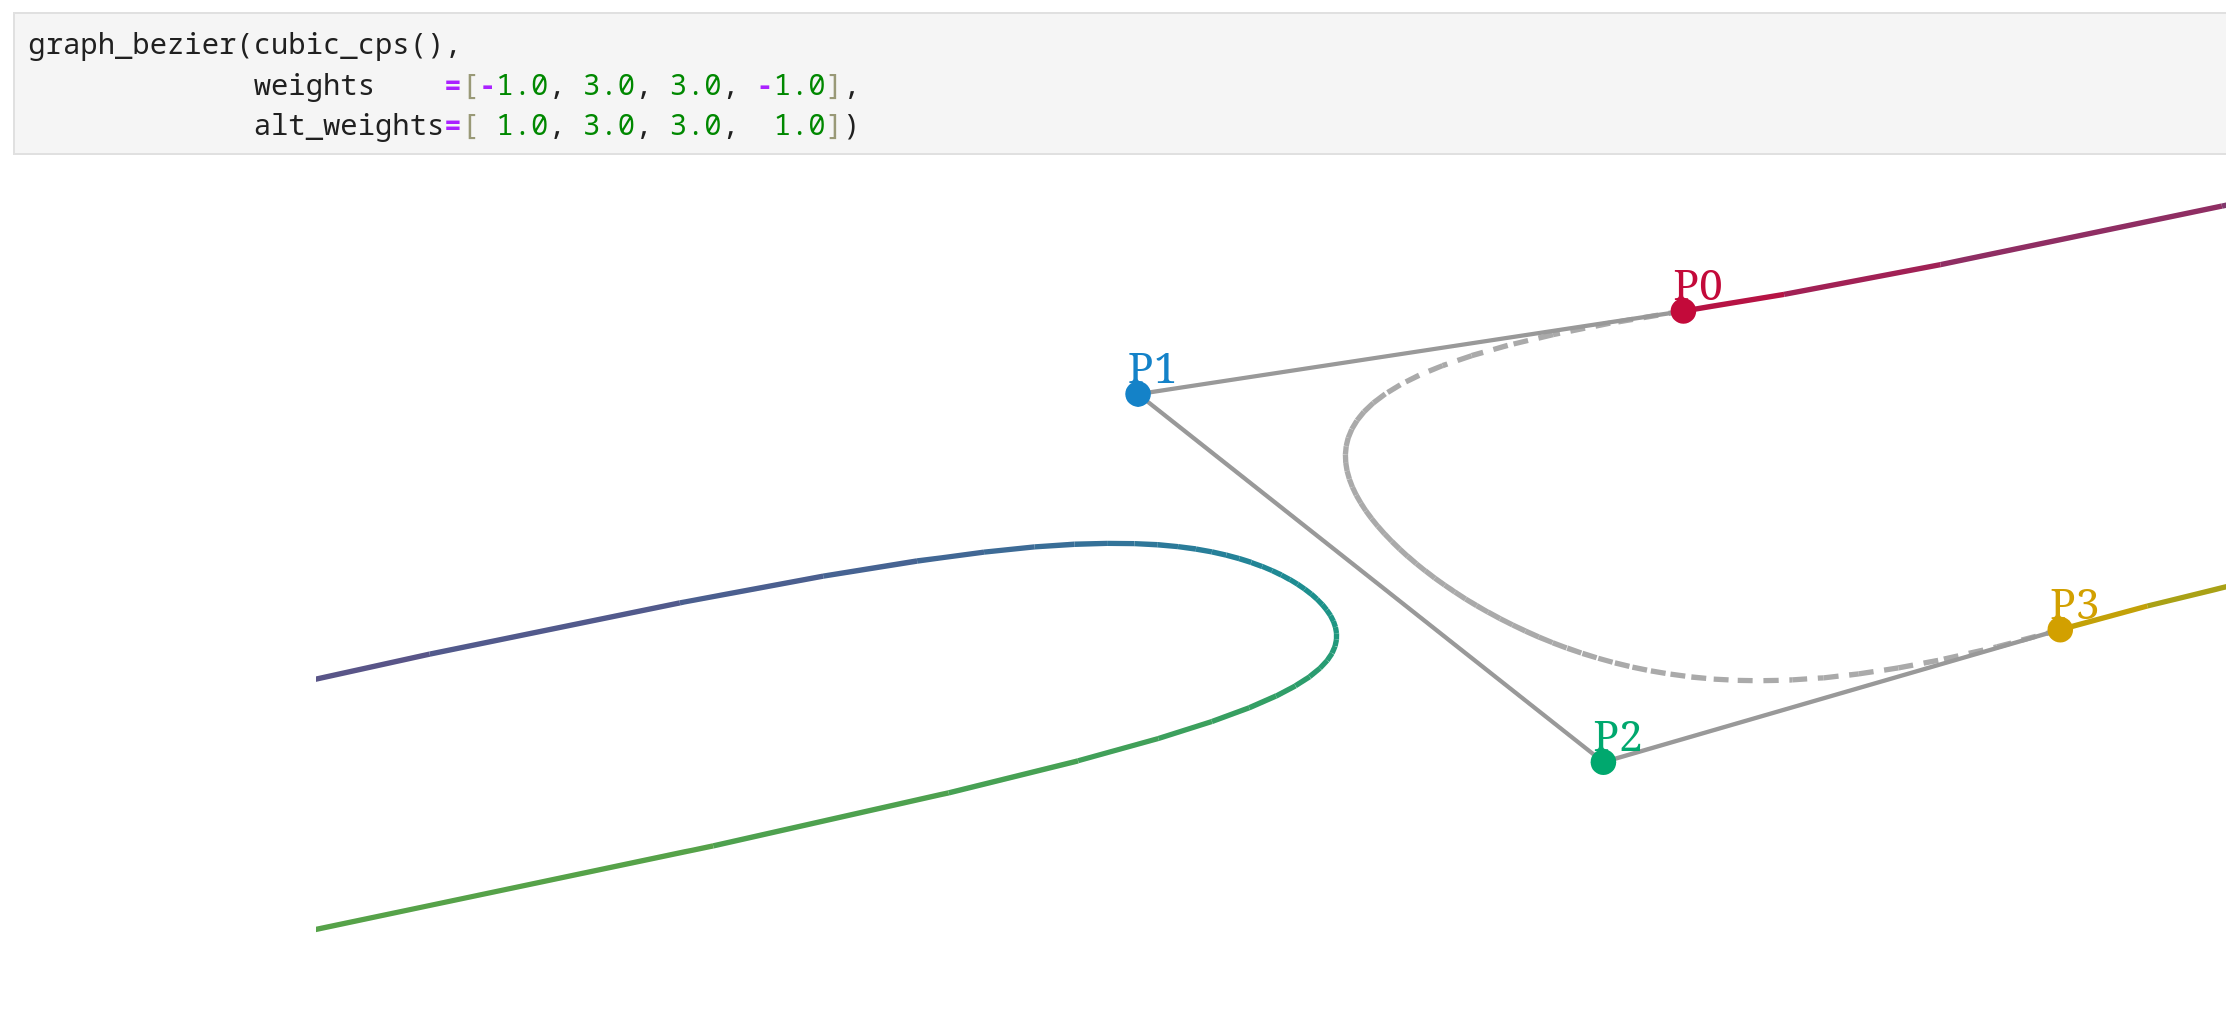
\includegraphics[width=0.50\linewidth]{figures/notebook.png}}}
    \end{center}
   % \hfill\href{https://eharquin.github.io/pga-bezier}{\beamergotobutton{Interactive notebooks}}
    \end{block}
    
    \begin{block}{Future work}
        \begin{itemize}\setlength\itemsep{0.1em}
            \item Using complex/versors weights $\lambda_i$
            \item Bézier surfaces and splines in PGA
            \item Geodesic versor interpolation (exp / log maps, ScLERP)
            % \item Integration into optimized GA libraries and CAD pipelines
        \end{itemize}
    \end{block}

\end{frame}
%%%%%%%%%%%%%%%%%%%%%%%%%%%%%%%%%%%%%%%%%%%%%%%%%%%%%%%%%%%%%%%%%%%%%%%%%%%%%%%%%%%%%%%%%%%%%%%%%


%%%%%%%%%%%%%%%%%%%%%%%%%%%%%%%%%%%%%%%%%%%%%%%%%%%%%%%%%%%%%%%%%%%%%%%%%%%%%%%%%%%%%%%%%%%%%%%%%
{\setbeamercolor{palette primary}{fg=black, bg=yellow}
  \begin{frame}[standout]
    Questions?
  \end{frame}
}
%%%%%%%%%%%%%%%%%%%%%%%%%%%%%%%%%%%%%%%%%%%%%%%%%%%%%%%%%%%%%%%%%%%%%%%%%%%%%%%%%%%%%%%%%%%%%%%%%


\end{document}
